\documentclass[11pt]{article}
\usepackage{geometry}
\geometry{a4paper}
\linespread{1.1} % Line spacing

% FIGURES AND FLOATS
\usepackage{graphicx} % Required for including pictures
\usepackage{float} % Allows putting an [H] in \begin{figure} to specify the exact location of the figure
\usepackage{wrapfig} % Allows in-line images such as the example fish picture
\usepackage[font={small,it}]{caption}
\usepackage{subcaption}
\usepackage{epstopdf}
\usepackage{pifont}

% MATH
\usepackage{amssymb}
\usepackage{amsmath}
\usepackage{algorithm}
\usepackage[noend]{algpseudocode}
\usepackage{bm}

% OTHER
\usepackage{color}
\usepackage{xeCJK}


%%%%%%%%%%%%%%%%%%%%%%%%%%%%%%%%%%%%%%%%%%%%%%%%%%%%%%%%%%%%
\title{一周学会Linux - 韩顺平}
\author{muyi}
\begin{document}
\maketitle


\section{Linux与Unix的关系}

\subsection{Unix}
\begin{figure}[htb]
    \centering
    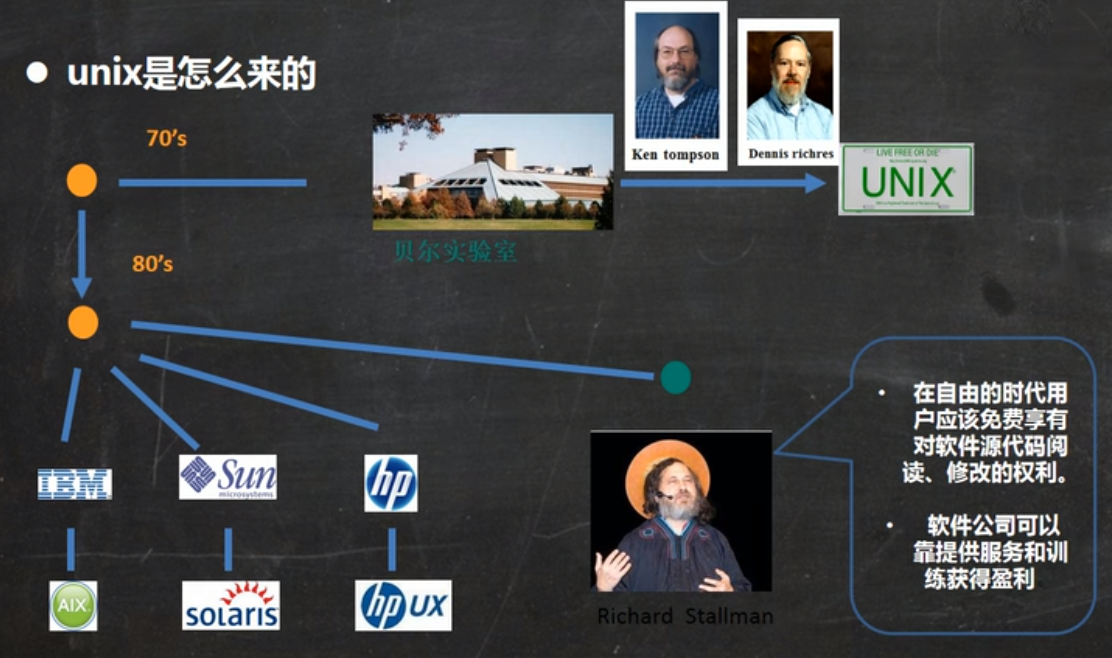
\includegraphics[scale=0.12]{imgs/unix.png}
\end{figure}

\subsection{Linux}
\begin{figure}[htb]
    \centering
    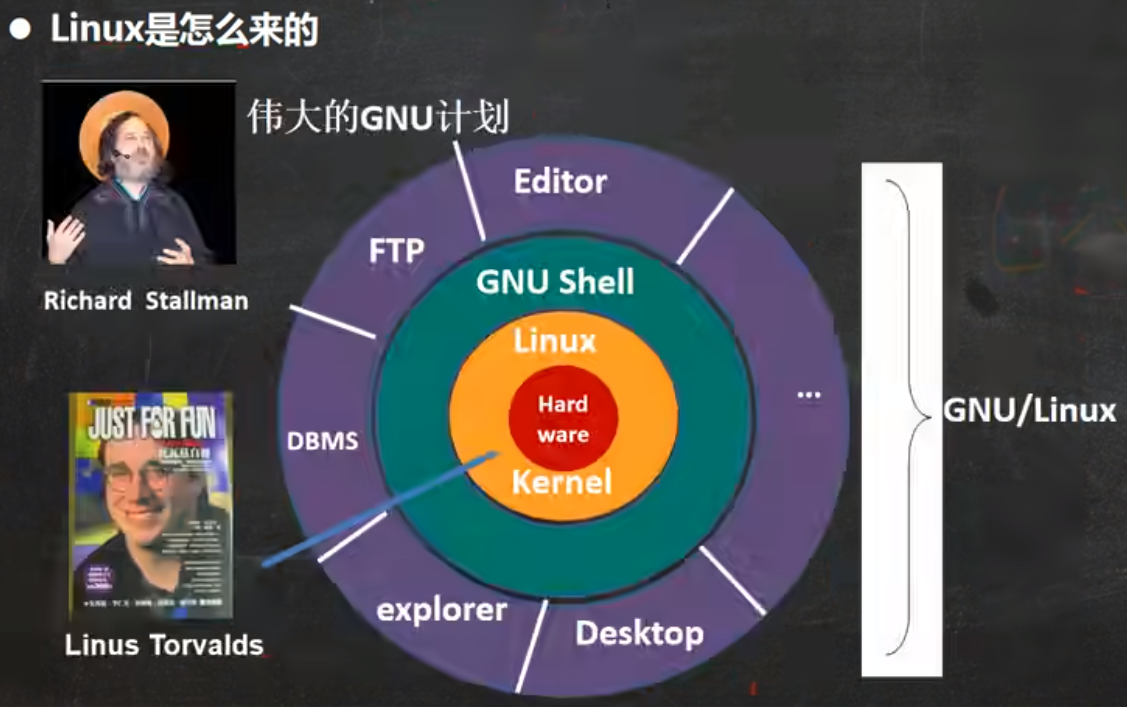
\includegraphics[scale=0.12]{imgs/gnu_linux.png}
\end{figure}

\subsection{Unix to Linux}
\begin{figure}[htb]
    \centering
    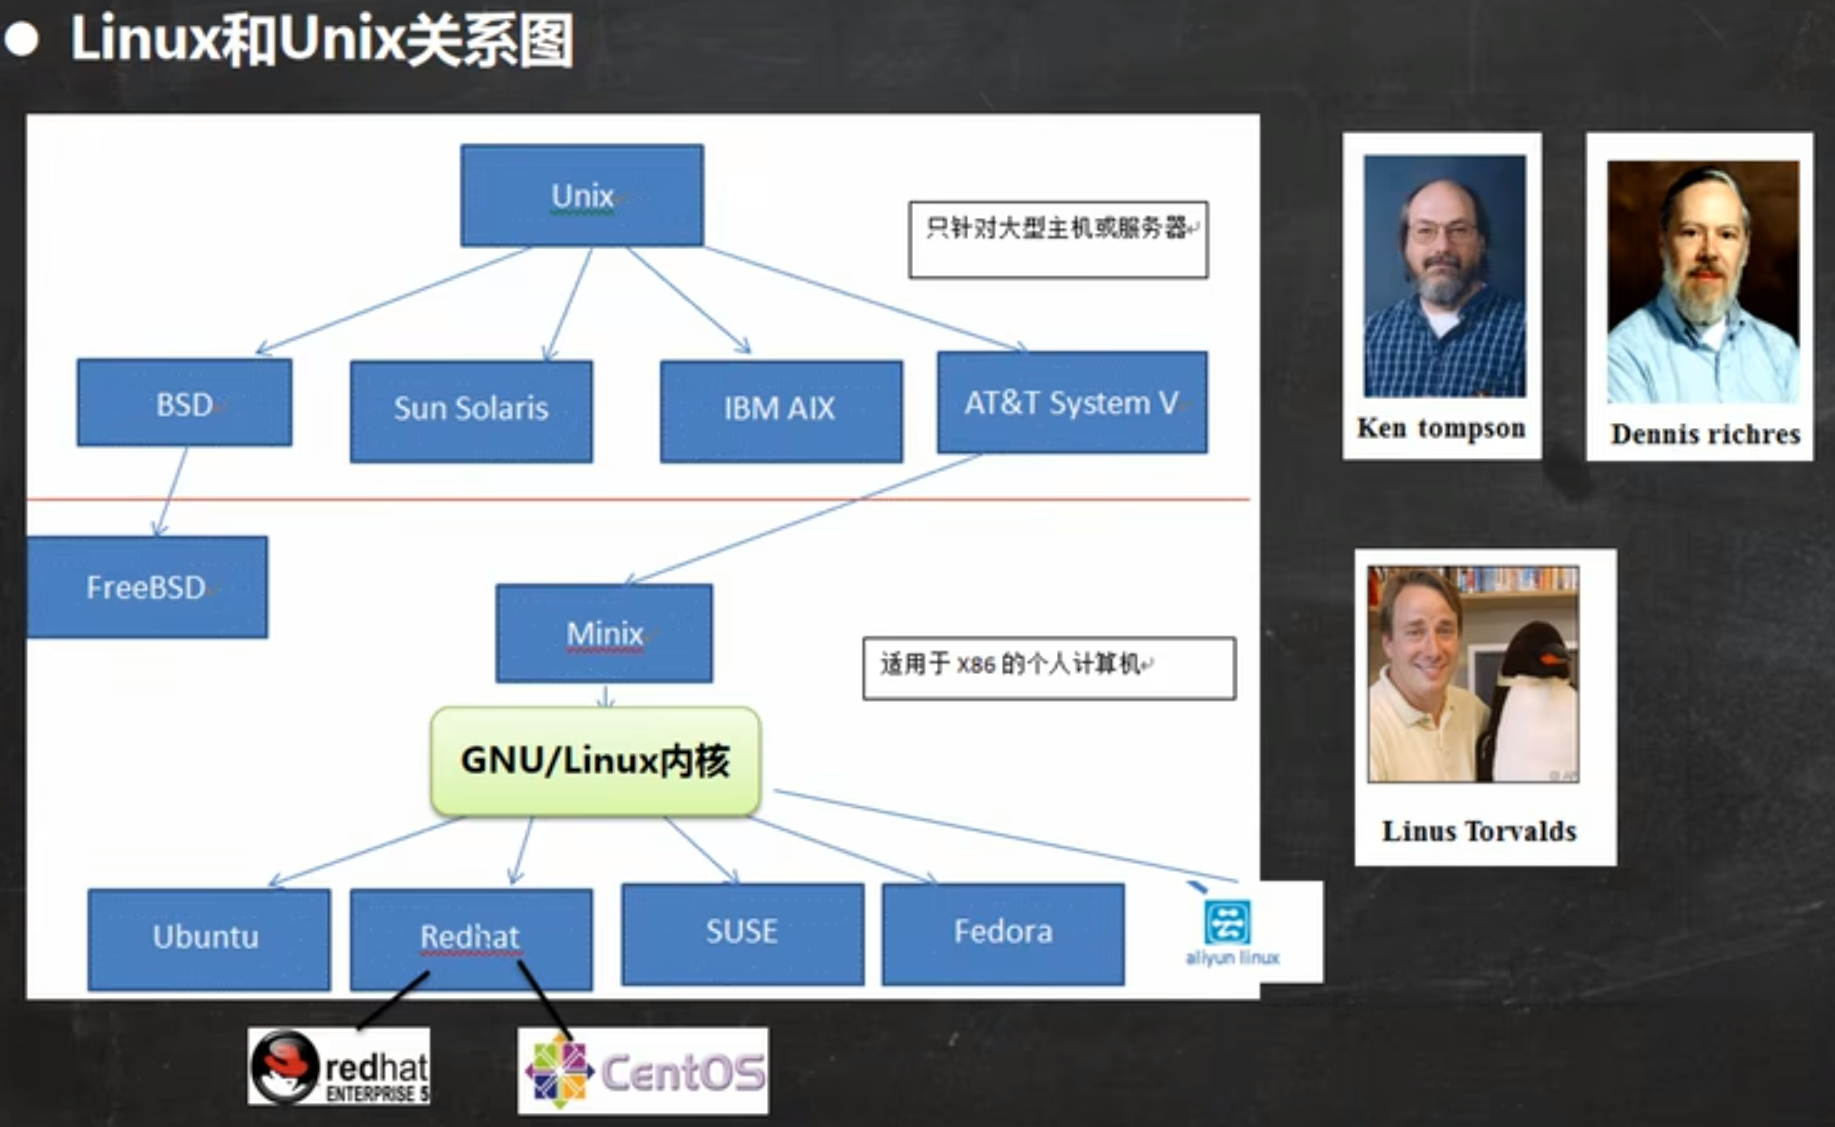
\includegraphics[scale=0.08]{imgs/unix_linux.png}
\end{figure}


\section{目录结构}
在Linux的世界里,一切皆文件。
\subsection{常见目录}
/:根目录  \\
/bin(/usr/bin, /usr/local/bin):存放常用命令  \\
/sbin(/usr/sbin, /usr/local/sbin):Super User管理员的命令  \\
/home:普通用户的主目录  \\
/root:管理员的主目录  \\
/lib:动态链接库  \\
/lost+found:当系统非法关机后这里会存放一些文件,一般为空  \\
/etc:配置文件  \\
/usr:应用程序  \\
/boot:启动文件  \\
/proc, /srv, /sys:系统相关的文件  \\
/tmp:临时文件  \\
/dev:类似设备管理器,对应硬件  \\
/media:U盘、光驱等  \\
/mnt:挂载别的文件系统  \\
/var:存放一些经常修改的内容,比如日志 \\


\section{Vim}

\subsection{三种模式}
\ding{172} 一般模式:用vim打开一个文件后就是一般模式,在此模式下可以使用复制、粘贴、删除整行等功能。  \\
\ding{173} 插入模式:在一般模式下输入i即可进入插入模式,在此模式下对文件进行编辑。  \\
\ding{174} 命令行模式:在插入模式下,先按esc键退出插入模式,然后输入:即可进入命令行模式(在一般模式下
直接输入:即可),在此模式下可以进行保存、退出、设置显示行号等操作。
\begin{figure}[htb]
    \centering
    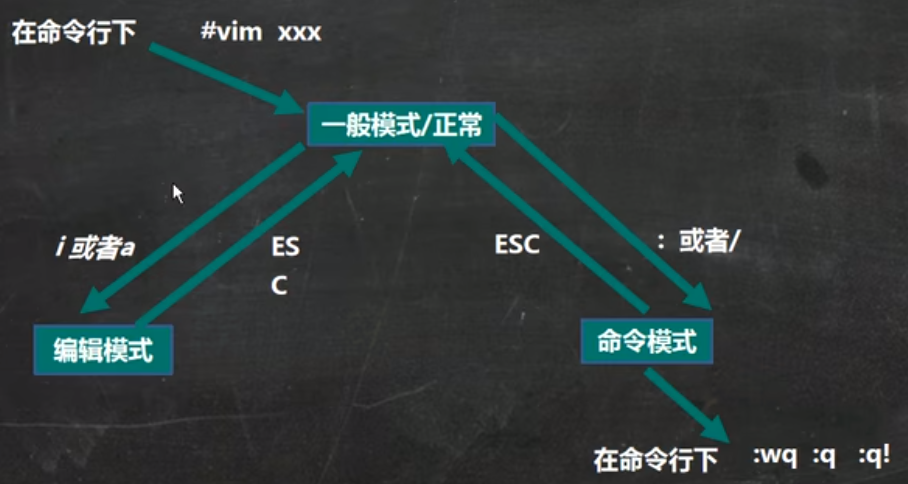
\includegraphics[scale=0.18]{imgs/vim_mode.png}
\end{figure}

\subsection{Vim快捷键}
复制当前行:\textbf{yy} \qquad 向下复制n行:\textbf{nyy} \qquad 粘贴:\textbf{p} \qquad
删除当前行:\textbf{dd} \qquad 向下删除n行:\textbf{ndd} \qquad 查找关键词:\textbf{
/keyword} \qquad 定位首行:\textbf{gg} \qquad 定位第n行:\textbf{ngg} \qquad 定位末行:
\textbf{G} \qquad 撤销:\textbf{u} \qquad 显示/不显示行号:\textbf{set nu/nonu}

\section{关机重启}

\subsection{关机}
最常用的关机命令是shutdown,用法如下: \\
\textbf{shutdown -h now} \qquad 马上关机 \qquad shutdown -h 5 \qquad 5分钟后关机 \\
\textbf{shutdown -r now} \qquad 马上重启 \\
除了shutdown之外这几个命令也可以关机,但有细微区别:\textbf{halt}, \textbf{poweroff}, \textbf{init 0}.

\subsection{重启}
\textbf{shutdown -r now} \quad 或 \quad \textbf{reboot}

\subsection{同步}
\textbf{sync}:把内存中的数据同步到磁盘  \\
一般在关机或重启前应当先运行sync命令以防数据丢失,但目前shutdown/reboot/halt等命令在关机前均会
先调用sync命令。

\subsection{运行级别}
0:关机 \qquad 1:单用户(可在此模式下找回密码) \qquad 2:多用户,但没有网络服务 \qquad 3:
多用户,且有网络服务 \qquad 4:系统保留 \qquad 5:图形界面 \qquad 6:系统重启  \\
常用的运行级别是3和5,通过init 0/1/2/3/4/5/6指令可以切换运行级别。

\section{用户管理}
添加用户:\textbf{useradd -m username}(带-m参数以自动生成/home/username目录) \\
修改用户密码:\textbf{passwd username} \\
删除用户:\textbf{userdel (-r) username}(不带-r参数时删除用户但保留/home/username文件夹,带-r参数则
连同文件夹一起删除) \\
查询用户信息:\textbf{id username} \\
切换用户:\textbf{su (-) username}(若不带-仅切换用户,带-同时将当前目录切换到/home/username) \\
新增用户组:\textbf{groupadd groupname} \\
删除用户组:\textbf{groupdel groupname} \\
修改用户所属组:\textbf{usermod -g groupname username}(在添加用户时可以通过-g参数直接指定所属组,即
\textbf{useradd -g groupname username},若没有指定组,则系统会自动新建一个和username同名的组) \\
相关文件:用户信息保存在/etc/passwd,密码信息保存在/etc/shadow,组的信息保存在/etc/group。

\section{常用指令}

\subsection{文件目录指令}

\textbf{pwd}:显示当前目录的绝对路径 \\
\textbf{ls}:显示当前目录下的文件(带-a参数显示隐藏文件,带-l参数以列表形式显示) \\
\textbf{mkdir (-p) dirname}:创建文件夹,带-p参数才能创建多级目录  \\
\textbf{rmdir dirname}:删除空目录 \qquad \textbf{rm -rf dirname}:删除非空目录  \\
\textbf{touch filename}:创建一个空文件 \\
\textbf{cp (-r) source dest}:拷贝文件(-r参数表示递归)  \\
\textbf{mv source/oldName dest/newName}:移动文件或者重命名文件  \\
\textbf{cat (-n) filename}:以只读方式查看文件(带-n参数显示行号)  \\
\textbf{less filename}:按页显示文件内容,适合用来查看较大的文件  \\
\textbf{echo}:输出内容到terminal,例如echo \$PATH查看环境变量 \\
\textbf{tail filename}:显示文件末尾10行 \qquad \textbf{tail -f filename}:实时监控文件内容更新 \\
\bm{$>$}和\bm{$>>$}:输出重定向,将本该输出到terminal的内容写入文件,例如echo 'something' > filename。
区别在于>是覆盖,$>>$是追加。  \\
\textbf{ln -s source dest}:创建软链接  \\
\textbf{history}:查看执行过的指令

\subsection{时间日期指令}
\textbf{date}:显示时间日期信息,也可通过添加参数格式化输出  \\
\textbf{cal}:显示本月日历

\subsection{搜索查找指令}
\textbf{find dirname -name filename}:在dirname目录下查找filename文件,输出其路径 \\
\textbf{locate filename}:功能和find类似,也是输出filename文件的路径,但locate指令比find指令快得多,
因为locate指令并不会真的扫描文件目录,而是在一个数据库中查找filename对应的路径。系统会每天自动
更新该数据库,所以如果用locate指令查找刚刚创建的文件会找不到,或者查找刚刚删除的文件仍显示出删除
前的路径。为避免这种情况,可以在locate前使用\textbf{updatedb}指令手动更新数据库。  \\
\textbf{which cmdname}:查看某个指令所在的路径,如\textbf{which ls}  \\
\textbf{grep}:搜索关键词,常和管道符号|一起使用,如\textbf{cat filename | grep keyword}

\subsection{压缩解压指令}
gzip/gunzip:\textbf{gzip filename}压缩文件(只能压缩为.gz),\textbf{gunzip filename.gz}解压文件  \\
zip/unzip:zip常用选项-r递归压缩,unzip常用选项-d指定解压文件存放目录  \\
tar:压缩用\textbf{tar -zcvf filename.tar.gz files2zip},解压用\textbf{tar -zxvf filename.tar.gz}

\section{组管理和权限管理}

\subsection{组管理}
$\bullet$ 在Linux中每个用户必须属于一个组,不能独立存在。对于Linux中的文件有所有者、所在组、其他组三个概念。  \\
$\bullet$ 通过\textbf{chown username filename}可以修改文件的所有者;通过chgrp groupname filename
可以修改文件所在组;通过\textbf{usermod -g groupname username}可以修改用户所属的组。

\subsection{rwx权限}
\ding{172} 当我们在某个路径下执行ls -l命令时,对于每个文件/目录,我们会得到类似下图所示的信息:
\begin{figure}[htb]
    \centering
    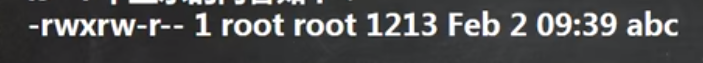
\includegraphics[scale=0.4]{imgs/rwx_info.png}
\end{figure}  \\
其中前10位(-rwxrw-r--)代表了该文件/目录的权限信息,具体含义如下:  \\
第1位(-、d、l、c、b)表示文件类型:-代表普通文件,d表示目录,l表示链接,c表示字符设备文件(键盘、
鼠标等),b表示块文件(硬盘等)。  \\
第2$\sim$4位表示该文件/目录所有者的权限。  \\
第5$\sim$7位表示该文件/目录所在组的权限。  \\
第8$\sim$10位表示该文件/目录其他组的权限。  \\
权限信息后的数字表示此目录下的子目录的个数(只算目录不算文件),如果是文件而非目录,则该数字为1。
对于目录还需要注意,因为任何一个目录默认包含./和../两个子目录,因此对一个空文件夹,该数字为2。\\\\
\ding{173} 文件的rwx权限:  \\
r:可以读取,查看;  \\
w:可以修改,但是不代表可以删除该文件,删除一个文件需要对该文件所在的目录拥有w权限;  \\
x:可以被执行。  \\\\
\ding{174} 目录的rwx权限:  \\
r:可以读取,即可以用ls查看内容;  \\
w:可以修改,即可以在目录内创建、删除文件或者重命名目录;  \\
x:可执行,即可以cd进入该目录。 \\\\
\ding{175} rwx也可以用数字来表示(r=4, w=2, x=1),因此rwx=4+2+1=7。

\subsection{修改rwx权限}
chmod:修改文件或目录的权限,具体使用方法如下。  \\
\ding{172} 通过u(所有者)、g(所在组)、o(其他用户)、a(所有用户)和+、-、=组合的方式修改权限。例如:
\textbf{chmod u=rwx,g=rx,o=r filename/dirname}, \quad \textbf{chmod u+x filename/dirname}等。\\
\ding{173} 通过数字修改权限。前文已经提到过,rwx也可以用数字来表示(r=4, w=2, x=1)。因此,
\textbf{chmod u=rwx,g=rx,o=r filename/dirname}也可以写成 \textbf{chmod 754 filename/dirname}。

\subsection{修改所有者和所在组}
修改所有者:\textbf{chown newowner filename/dirname} \\
修改所有者和所在组:\textbf{chown newowner:newgroup filename/dirname}  \\
修改所在组:\textbf{chgrp newgroup filename/dirname}


\section{定时任务调度}

\subsection{crond任务调度}
基本语法:\textbf{crontab [option]}  \\
e:编辑crontab定时任务 \qquad l:列出crontab任务 \qquad r:删除当前用户的所有crontab任务 \\
时间格式:m(minute) h(hour) dom(dayOfMonth) mon(month) dow(dayOfWeek)  \\
\begin{figure}[htb]
    \centering
    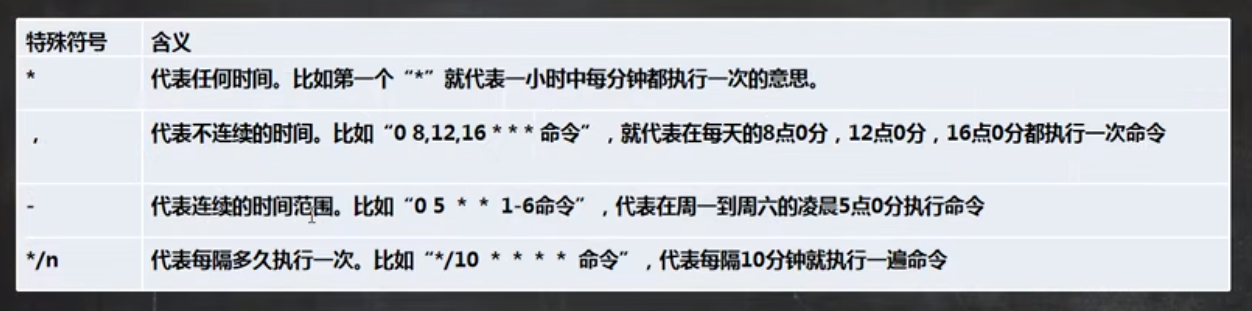
\includegraphics[scale=0.3]{imgs/crontab.png}
\end{figure} \\
使用crond定时执行脚本时,要确认对该脚本有执行权限。  \\
重启crond服务:\textbf{service crond restart}

\subsection{at定时任务}
at指令是一次性定时任务,执行完一次后便不再执行。at的守护进程atd会以后台模式运行,默认情况下atd守护
进程每60s检查一次作业队列。在使用at指令时,一定要保证atd进程已启动。  \\
at命令格式:\textbf{at [option] [time]}  \\
\begin{figure}[htb]
    \centering
    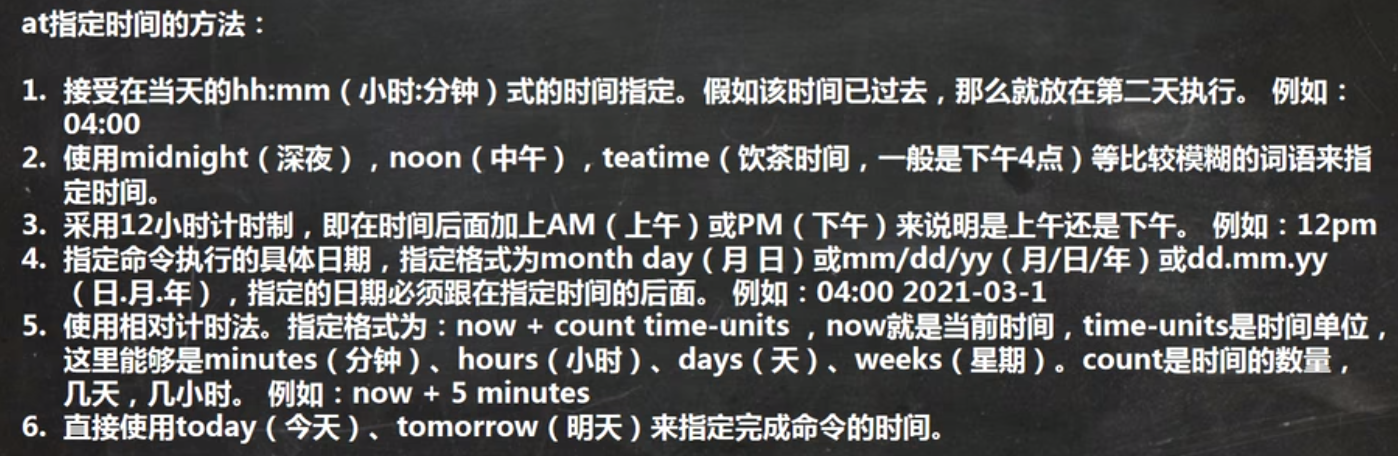
\includegraphics[scale=0.27]{imgs/at_time.png}
\end{figure} \\
用\textbf{atq}命令可以查看还未执行的任务,用\textbf{atrm+任务编号}可以删除任务。

\section{磁盘和分区}
\subsection{分区}
$\bullet$ Linux的文件目录结构是独立且唯一的,比如只有一个根目录/,在根目录下面有一些必须的目录等。
Linux通过“载入”的方式将磁盘的一个分区和一个目录联系起来,这个目录就叫这个分区的挂载点。 \\
\begin{figure}[htb]
    \centering
    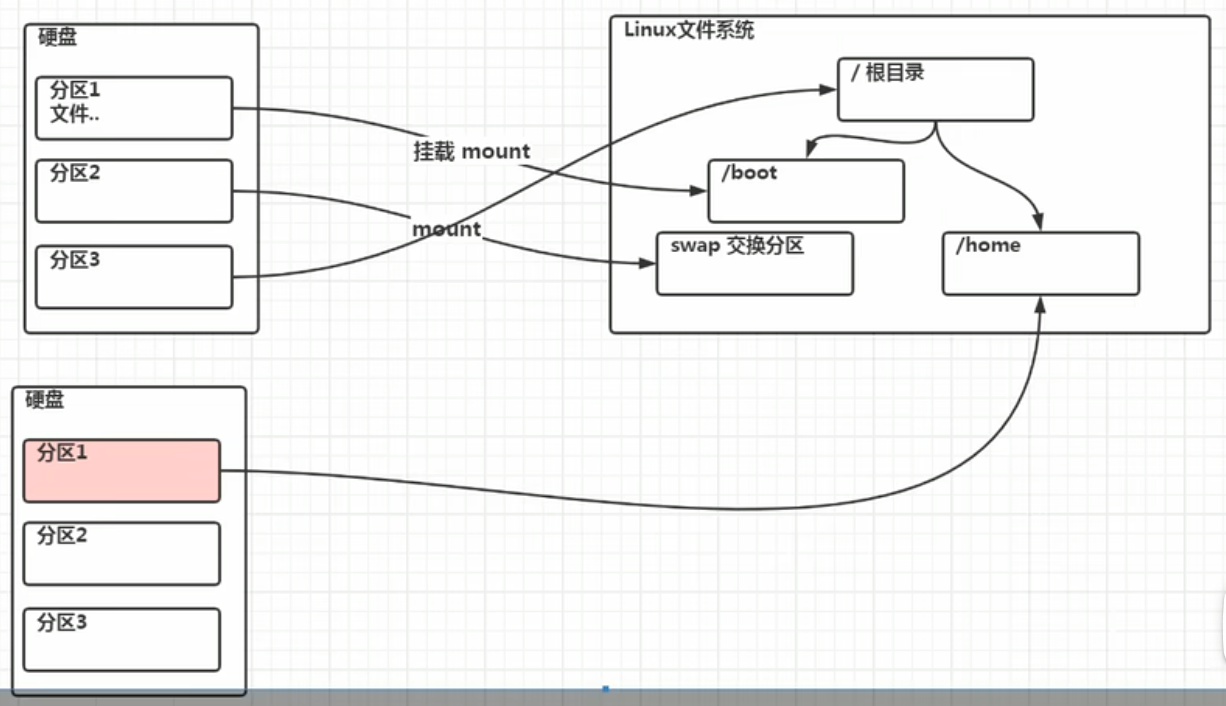
\includegraphics[scale=0.27]{imgs/parts.png}
\end{figure} \\
$\bullet$ Linux硬盘分为IDE硬盘和SCSI硬盘,目前基本是SCSI硬盘。 \\
对于IDE硬盘,驱动器标识符为hdx$\sim$。其中hd表示IDE硬盘;x为盘号(a为基本盘,b为基本从属盘,c为辅助
主盘,d为辅助从属盘);~表示分区,前四个分区用数字1到4表示他们是主分区或扩展分区,从5开始是逻辑
分区。例如:hda3,hdb2。\\
SCSI硬盘的驱动器标识符格式为sdx~,其中sd表示SCSI硬盘,其余部分的含义与IDE硬盘相同。
\\
$\bullet$ 查看设备挂载情况:\textbf{lsblk} 或 \textbf{lsblk -f}(可以显示UUID)

\subsection{增加硬盘并挂载}
磁盘分区:\textbf{fdisk /dev/sdx}(根据实际情况看是sdb还是sdc还是sdd等等),在分区最后需要输入w使分区生效  \\
格式化分区:\textbf{mkfs -t ext4 /dev/sdx$\sim$}  \\
挂载:\textbf{mount [分区名称] [挂载点]},例如 mount /dev/sdb1 /newdisk  \\
卸载:\textbf{umount [分区名称]} 或 \textbf{umount [挂载点]}  \\
注意,使用mount挂载的分区重启后会失效,如果需要开机时自动挂载,需要修改/etc/fstab文件。

\subsection{磁盘查询}
$\bullet$ 查询系统磁盘整体使用情况:\textbf{df -h}  \\
$\bullet$ 查询某个文件或某个目录的磁盘使用情况:\textbf{du -h filename/dirname}  \\
$\bullet$ 用树状形式显示目录结构:\textbf{tree dirname}

\section{网络配置}
查看网络配置信息:\textbf{ifconfig} \\
测试主机之间网络连通性:\textbf{ping 目的主机} \\
配置静态IP:修改/etc/netplan/01-network-manager-all.yaml文件 \\
\begin{figure}[htb]
    \centering
    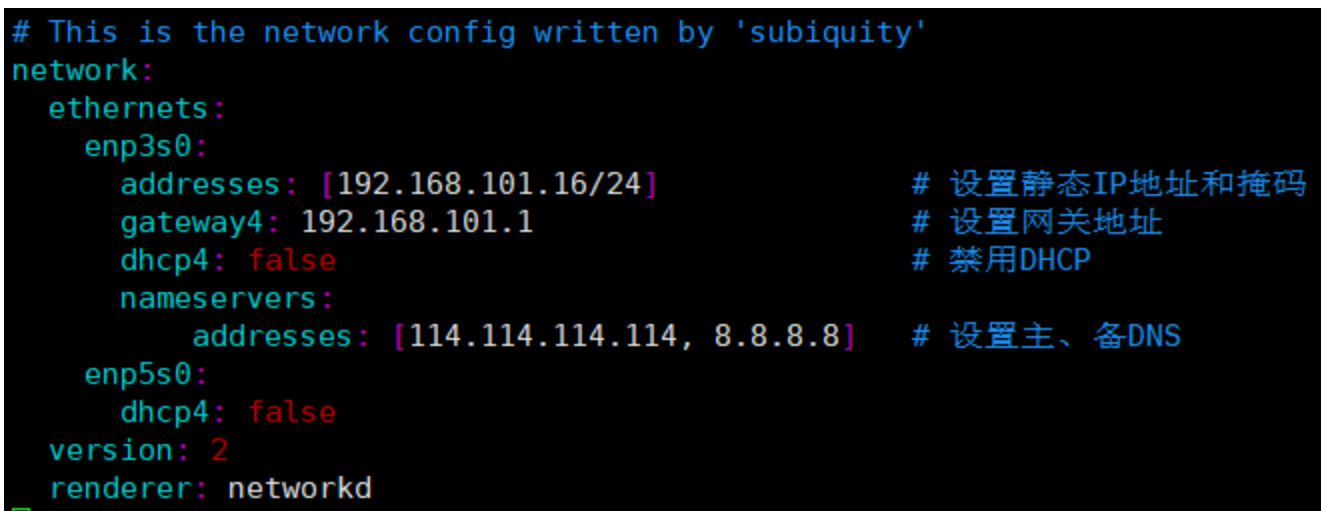
\includegraphics[scale=0.27]{imgs/static_ip.png}
\end{figure} \\
修改完之后用\textbf{sudo netplan apply}应用网络配置。 \\
查看当前主机名:\textbf{hostname} \qquad 修改主机名:编辑/etc/hostname文件 \qquad 设置hosts映射:
编辑/etc/hosts文件

\section{进程管理}
\subsection{基础}
查看进程信息:\textbf{ps -aux} 或 \textbf{ps -ef}(显示内容略有不同)  \\
通过pid终止进程:\textbf{kill [-9] pid}(选项-9表示强制终止,可以不带) \\
通过进程名终止进程:\textbf{killall 进程名}(支持通配符) \\
查看进程树:\textbf{pstree [-pu]}(选项p表示显示进程的pid,选项u表示显示进程的所属用户)

\subsection{服务管理}
\begin{enumerate}
\item 定义:服务(service)本质上就是进程,但是是运行在后台的,通常会监听某个端口,等待其他程序的
请求,因此又称为守护进程,比如mysqld、sshd、防火墙等。 \\
\item 服务管理指令:\textbf{service serviceName start|stop|restart|reload|status}  \\
\item 查看系统运行级别(runlevel):\textbf{systemctl get-default} \quad 设置系统运行级别:
\textbf{systemctl set-default TARGET.target}。常用的运行级别是3(multi-user.target)和5(
graphical.target)。  \\
\item chkconfig指令:设置某个服务在某个运行级别是否自启动。 \\
\textbf{chkconfig --list} \quad 查看chkconfig管理的服务  \\
\textbf{chkconfig --level 3/5 serviceName on/off} \quad 设置某服务在3/5运行级别下是否自启动 \\
通过chkconfig设置后需要重启才能生效。
\item 除了service指令外,其实更多的服务是通过systemctl指令进行管理的,相关的命令如下:
\begin{description}
    \item[systemctl start|stop|restart|status serviceName] 启动/停止/重启/查看某服务
    \item[systemctl list-unit-files] 查看所有服务的自启动设置
    \item[systemctl enable serviceName] 设置某服务为开机自启动
    \item[systemctl disable serviceName] 关闭某服务开机自启动
    \item[systemctl is-enabled serviceName] 查询某服务是否是开机自启动
\end{description}
\item 打开或关闭指定的端口(firewall指令)
\begin{description}
    \item[firewall-cmd --permanent --add-port=port/protocol] 打开端口
    \item[firewall-cmd --permanent --remove-port=port/protocol] 关闭端口
    \item[firewall-cmd --reload] 打开或关闭端口后,reload以使其生效
    \item[firewall-cmd --query-port=port/protocol] 查询某端口是否打开
\end{description}
\item 在ubuntu系统中,默认的防火墙软件是ufw,因此通过ufw指令来管理端口,常用指令如下:
\begin{description}
    \item[ufw enable] 启动ufw
    \item[ufw disable] 停止ufw
    \item[ufw status] 查询ufw状态
    \item[ufw allow port/protocol] 打开端口(由于ufw默认配置了一些常用协议对应的端口,因此
    也可以只写port或者protocol)
    \item [ufw deny port/protocol] 关闭端口
    \item [ufw delete allow/deny port/protocol] 删除打开/关闭某个端口的规则
\end{description}
\item top命令和ps命令类似,都是用来查看进程信息,但top命令显示的信息可以每隔一段时间自动更新,
常用用法如下:
\begin{description}
    \item[top -d 5] 每隔5秒自动更新,如果不带数字直接top -d则默认每隔3秒更新
    \item[top -i] 不显示idel和zombie进程
    \item[top -p pid] 通过指定pid来单独监控某个进程
\end{description}
\item top交互操作
\begin{description}
    \item[输入P] 按CPU占用率排序
    \item[输入M] 按内存占用率排序
    \item[输入N] 按PID排序
    \item[输入u,然后输入用户名] 按用户查看进程
    \item[输入k,然后输入PID,然后输入9] kill某个进程
    \item[输入q] 退出top
\end{description}
\item \textbf{netstat -anp} 查看系统的网络连接情况
\end{enumerate}

\section{软件包管理}
\begin{enumerate}
    \item rpm包:SUSE、RedHat、CentOS等采用
    \begin{description}
        \item[rpm -qa] 查询安装的全部rpm包
        \item[rpm -q pkgName] 查询是否安装了某个软件包
        \item[rpm -qi pkgName] 查询某个软件包的详细信息
        \item[rpm -qf path] 查询某个文件所属的软件包
        \item[rpm -e pkgName] 卸载rpm包
        \item[rpm -ivh pkgPath] 安装rpm包
    \end{description}
    \item yum:rpm软件包的包管理器,能够从指定的服务器自动下载rpm包并安装,而且自动处理依赖关系。
\end{enumerate}

\section{Shell编程}
\subsection{Shell入门}
Shell是一个命令解释器,它为用户提供了一个向Linux内核发送请求以便运行程序的界面系统级程序,用户
可以通过Shell来启动、挂起、停止甚至是编写一些程序。
\begin{figure}[htb]
    \centering
    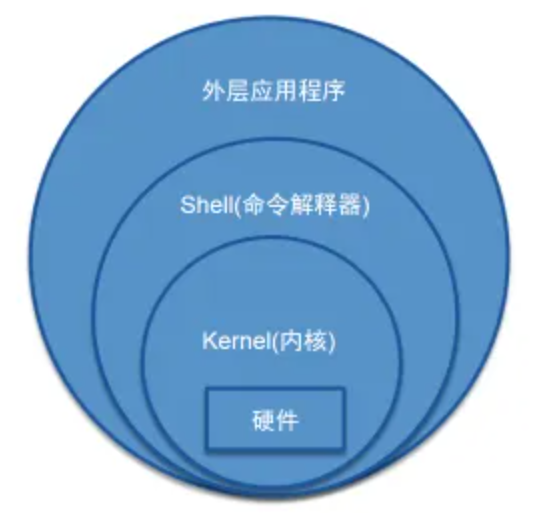
\includegraphics[scale=0.3]{imgs/shell.png}
\end{figure}  \\
Shell脚本以\textbf{\#!/bin/bash}开头,以指明使用的Shell。当直接执行脚本时,需要先给脚本赋予
执行权限,当使用\textbf{sh}执行时则不用赋予执行权限。

\subsection{Shell变量}
\begin{enumerate}
\item Linux Shell中的变量分为系统变量和用户自定义变量,常见的系统变量如\#HOME,\#SHELL,\#USER,
\#PATH等,使用\textbf{set}命令可以查看所有的系统变量。
\item 自定义变量
\begin{description}
    \item 定义变量:\textbf{变量名=值}(注意=前后不要有空格)
    \item 撤销变量:\textbf{unset 变量名}
    \item 声明静态变量:\textbf{readonly 变量名=值}(注意,静态变量不能被unset)
\end{description}
\item 变量名称可以由字母、数字和下划线组成,但不能以数字开头;变量名称一般习惯大写。
\item 将命令的返回值赋给变量:使用反引号(例如\textbf{A=$\grave{}$date$\grave{}$})或使用
$\$$()(例如\textbf{A=\$(date)})。
\end{enumerate}

\subsection{设置环境变量}
\textbf{export VarName=Value}:将Shell变量输出为环境变量/全局变量 \\
\textbf{source configFile}:使修改后的环境变量生效 \\
\textbf{echo \$Var}:查询某个环境变量的值 \\
Shell脚本中多行注释的写法:\textbf{:$<<$! code !}

\subsection{位置参数变量}
\begin{enumerate}
    \item 当一个Shell脚本需要从外部获取参数时,需要用到位置参数变量,例如
    ./myshell.sh 100 200,相关用法如下:
    \begin{description}
        \item[\$n] n为数字,\$0为命令本身,\$1$\sim$\$9代表第一到第九个参数,第十个及以后
        的参数需要用大括号包含,比如\$\{10\}。
        \item[\$*] 代表所有的参数,当直接使用\$*时,每个参数独立;当被双引号包围,即"\$*"时,
        全部参数作为一个整体。
        \item[\$@] 代表全部参数,不论是否使用双引号每个参数始终独立。
        \item[\$\#] 代表参数的个数。
    \end{description}
\end{enumerate}

\subsection{预定义变量}
\begin{enumerate}
    \item 预定义变量是Shell语言预先定义好的变量,可以在Shell脚本中直接使用。常用的预定义变量如下:
    \begin{description}
        \item[\$\$] 获取当前进程的PID。
        \item[\$!] 获取后台运行的最后一个进程的PID。
        \item[\$?] 获取最后一次执行的命令的执行结果,若为0表示命令正确执行,若为非0值表示命令
        没有正确执行,可以结合C++中函数最后的return 0来理解。
    \end{description}
\end{enumerate}

\subsection{运算符与表达式}
\begin{enumerate}
    \item Shell中进行算数运算有下面三种写法:
    \begin{description}
        \item[\$((expr))] 注意必须要用两层括号把表达式包起来,例如\$(((2+3)*4))。
        \item[\$[expr]] 中括号里面可以使用小括号,但是最外层需要用中括号包起来,例如\$[(2+3)*4]。
        \item[expr m + n] 采用这种方式运算符前后必须有空格;如果要将计算结果赋给一个变量需要
        将整个表达式用反引号$\grave{}$ $\grave{}$包起来,包括expr本身;可用运算符有加$+$减$-$
        乘$\backslash$$*$除/和取余$\%$,注意乘号要用转义符。举例:RES=
        $\grave{}$ expr 2 + 3 $\grave{}$。
    \end{description}
\end{enumerate}

\subsection{条件判断与流程控制}
\begin{enumerate}
    \item 基本语法:\\
    \textbf{
        if [\quad condition \quad]  \\
        then \\
        some code... \\
        elif [\quad condition \quad]\\
        then \\
        some code... \\
        fi
    } \\
    注意中括号里面condition前后必须有空格。
    \item 字符串比较用\textbf{=},例如:if [\quad "ok" = "ok" \quad]
    \item 两个整数比较 \\
    \textbf{-lt} 小于 \qquad \textbf{-le} 小于等于 \qquad \textbf{-eq} 等于 \qquad
    \textbf{-gt} 大于 \qquad \textbf{-ge} 大于等于 \qquad \textbf{-ne} 不等于 \\
    例如:if [\quad 20 -ge 23 \quad]
    \item 判断文件权限 \\
    \textbf{-r} 有读权限 \qquad \textbf{-w} 有写权限 \qquad \textbf{-x} 有执行权限 \\
    例如:if [\quad -w abc.txt \quad]
    \item 判断文件是否存在 \\
    \textbf{-f} 文件存在且是一个普通文件 \qquad \textbf{-e} 文件存在 \qquad \textbf{-d}
    文件存在且是一个目录 \\
    例如:if [\quad -f abc.txt \quad]
\end{enumerate}

















    
\end{document}